\documentclass{beamer}
\usepackage[utf8]{inputenc}
\usepackage{graphicx}

\newtheorem{definicion1}{Posibles definiciones de $\pi$}
\newtheorem{definicion}{Definición}
\newtheorem{ejemplo}{Ejemplo}

%%%%%%%%%%%%%%%%%%%%%%%%%%%%%%%%%%%%%%%%%%%%%%%%%%%%%%%%%%%%%%%%%%%%%%%%%%%%%%%

\title[Curiosidades sobre $\pi$]{Curiosidades sobre el número $\pi$}
\author[Alba Crespo]{\textbf{Alba Crespo Pérez}}
\institute[ULL]{}
\date[23-04-2014]{23 de abril de 2014}

%%%%%%%%%%%%%%%%%%%%%%%%%%%%%%%%%%%%%%%%%%%%%%%%%%%%%%%%%%%%%%%%%%%%%%%%%%%%%%%

\usetheme{Madrid}
\usecolortheme{crane}

%%%%%%%%%%%%%%%%%%%%%%%%%%%%%%%%%%%%%%%%%%%%%%%%%%%%%%%%%%%%%%%%%%%%%%%%%%%%%%%

\begin{document}
  
%++++++++++++++++++++++++++++++++++++++++++++++++++++++++++++++++++++++++++++++
  
\begin{frame}

  
\includegraphics[width=0.15\textwidth]{img/ullesc.png}
  \hspace*{7.0cm}
  
\includegraphics[width=0.16\textwidth]{img/fmatesc.png}
  \titlepage

  \begin{small}
    \begin{center}
      \emph{Facultad de Matemáticas} \\
      Universidad de La Laguna
    \end{center}
  \end{small}

\end{frame}

%++++++++++++++++++++++++++++++++++++++++++++++++++++++++++++++++++++++++++++++  

%++++++++++++++++++++++++++++++++++++++++++++++++++++++++++++++++++++++++++++++  

\begin{frame}
  \frametitle{Índice}  
  \tableofcontents[pausesections]
\end{frame}

%++++++++++++++++++++++++++++++++++++++++++++++++++++++++++++++++++++++++++++++  

\section{Características generales de $\pi$}

%++++++++++++++++++++++++++++++++++++++++++++++++++++++++++++++++++++++++++++++  

\subsection{Definición matemática}
\begin{frame}
\frametitle{1.1 Características generales: definición matemática}
\begin{block}{Posibles definiciones de $\pi$}

La definición más común de $\pi$ establece que su valor correponde a la 
\textbf{relación} existente \textbf{entre la longitud de una circunferencia 
y su diámetro}. \pause En consecuencia, $\pi$ es también el área de un círculo 
unitario en el plano euclídeo, así como el menor número real positivo que 
verifica la ecuación $sen(x) = 0$. De igual forma, es posible proporcionar 
\textbf{dos definiciones analíticas} de esta ubicua constante matemática: \pause 

\begin{itemize}
    \item 
      Equivale a la menor solución de la siguiente ecuación compleja: 
      \begin{center}
      $\boldsymbol{e^{ix} + 1 = 0}$
      \end{center}
      \pause
    \item
      La ecuación diferencial $\textbf{S''(x) + S(x) = 0}$, para la que existe solución
      única bajo las condiciones de contorno $S(0) = 0$ y $S'(0) = 1$, tiene
      como raíz positiva más pequeña al número $\pi$.
\end{itemize}

\end{block}
\end{frame}

%++++++++++++++++++++++++++++++++++++++++++++++++++++++++++++++++++++++++++++++

\subsection{$\pi$ como irracional y trascendente}
\begin{frame}
\frametitle{1.2. Carácter irracional y trascendente de $\pi$}

El carácter \textbf{irracional} de $\pi$ implica que \emph{no puede ser expresado a 
modo de cociente entre dos números enteros}, tal y como fue demostrado por Johann H. 
Lambert en 1761. \par \pause
Se trata además de un número \textbf{trascendente}, es decir, que \emph{no corresponde 
a la raíz de ningún polinomio de coeficientes enteros}, hecho que fue probado por el 
matemático alemán F. Lindemann durante el siglo XIX cerrando con ello una dilatada 
investigación acerca del histórico problema de la \textbf{cuadratura del círculo}, 
carente de solución (véase \cite{hist_pi}). Uno de los métodos empleados para la 
aproximación de $\pi$ viene dado por la integral: \pause

\setbeamertemplate{caption}{\insertcaption}
\begin{figure}[!th]
\begin{center}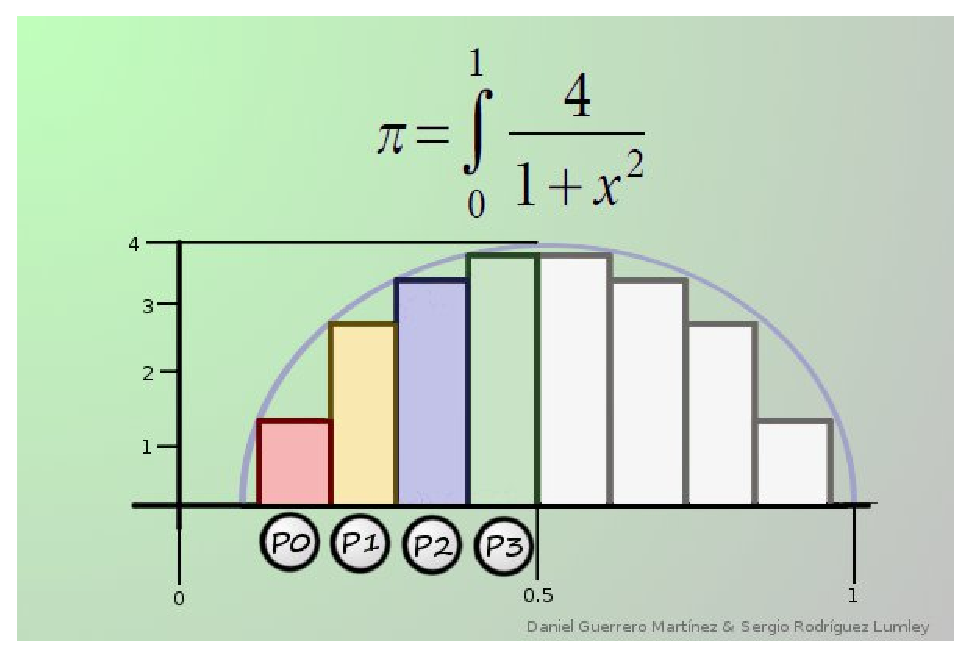
\includegraphics[height=2.5cm, width=5cm]{img/aprox.eps}
\caption{Figura 1: Integración para el cálculo de $\pi$.}
\label{int}
\end{center}
\end{figure}

\end{frame}

%++++++++++++++++++++++++++++++++++++++++++++++++++++++++++++++++++++++++++++++  

\section{Historia del número $\pi$}
\subsection{Aproximaciones hasta la Edad Moderna}

%++++++++++++++++++++++++++++++++++++++++++++++++++++++++++++++++++++++++++++++  

\begin{frame}
\frametitle{2.1. Descubrimiento histórico de $\pi$}
\begin{block}{Aproximaciones de $\pi$ hasta finales de la Edad Media}

\begin{table}[!ht]
\begin{center}
\begin{tabular}{|l|l|c|c|r|}
\hline
\textbf{AÑO} & \textbf{MATEMÁTICO O DOCUMENTO}   & \textbf{ERROR}  \\ \hline
1900 a.C.    & Papiro de Ahmes                   & 6016 ppm        \\ \hline
1600 a.C.    & Tablilla de Susa                  & 5282 ppm        \\ \hline
500 a.C.     & Bandhayana                        & 16422 ppm       \\ \hline
250 a.C.     & Arquímedes de Siracusa            & 13.15 ppm       \\ \hline
150 d.C      & Claudio Ptolomeo                  & 23.56 ppm       \\ \hline
263 d.C      & Wang Fan                          & 507 ppm         \\ \hline
300 d.C      & Chang Hong                        & 6584 ppm        \\ \hline
500 d.C      & Aryabhata                         & 2.34 ppm        \\ \hline
600 d.C      & Brahmagupta                       & 6584 ppm        \\ \hline
800 d.C      & Al-Jwarizmi                       & 2.34 ppm        \\ \hline
1220 d.C     & Fibonacci                         & 72.73 ppm       \\ \hline
1400 d.C     & Madhava                           & 0.085 ppm       \\ \hline
1424 d.C     & Al-Kashi                          & 0.1 ppm         \\ \hline

\end{tabular}
\end{center}
\label{history}
\end{table}

\end{block}
\end{frame}

%++++++++++++++++++++++++++++++++++++++++++++++++++++++++++++++++++++++++++++++

\subsection{Origen y popularidad de su simbología}
\begin{frame}
\frametitle{2.2 Influencia de Leonhard Euler}

El símbolo actual para la representación de $\pi$ fue adoptado por primera vez en 1706 
por el matemático \textbf{William Jones}, si bien la gran popularidad de esta convención 
vendría de la mano del destacado matemático y físico suizo \textbf{Leonhard Euler} (ver 
figura \ref{euler}). \par \pause Euler realizó importantes descubrimientos en áreas tan 
diversas como \textbf{astronomía}, \textbf{cálculo}, \textbf{teoría de grafos}, \textbf{mecánica} 
y \textbf{óptica}, siendo responsable de la introducción de gran parte de la moderna terminología 
y notación matemática. Se trata del \textbf{principal matemático del siglo XVIII} y uno de los 
más grandes y prolíficos de todos los tiempos. \pause

\setbeamertemplate{caption}{\insertcaption}
\begin{figure}[!th]
\begin{center}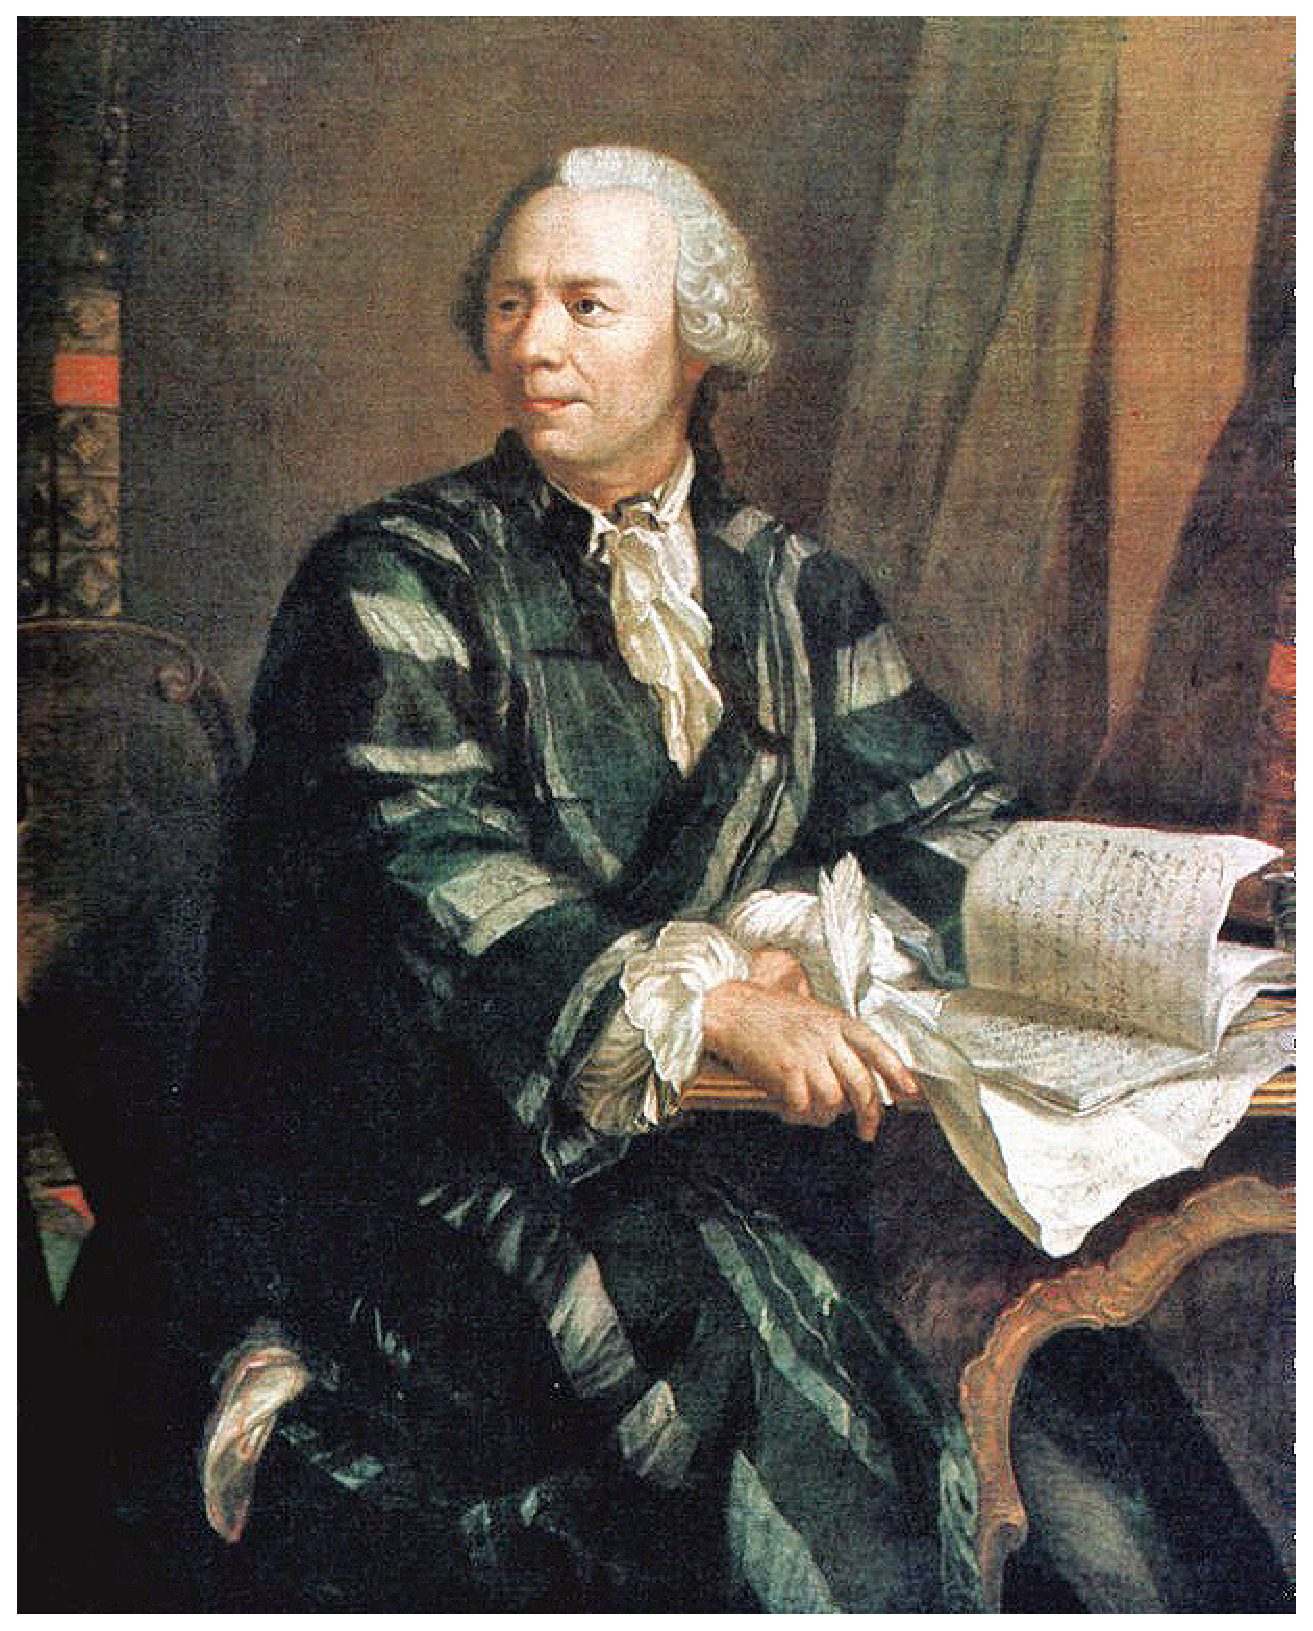
\includegraphics[height=2.5cm, width=2cm]{img/euler.eps}
\caption{Figura 2: Leonhard Euler}
\label{euler}
\end{center}
\end{figure}

\end{frame}

%++++++++++++++++++++++++++++++++++++++++++++++++++++++++++++++++++++++++++++++  

\section{Presencia de $\pi$ en las ciencias físicas}

%++++++++++++++++++++++++++++++++++++++++++++++++++++++++++++++++++++++++++++++  

\begin{frame}
\frametitle{3. La constante $\pi$ en el mundo real...}
\begin{block}{Magnitudes y leyes físicas que involucran a $\pi$}

\begin{itemize}
    \item 
      La expresión de la \textbf{constante cosmológica}: 
      \begin{center}
      $\Lambda = \frac{8 \pi G}{3 c^{2}}$
      \end{center}
      \pause
    \item
      El \textbf{principio de incertidumbre} de Heisenberg:
      \begin{center}
      $\Delta x \Delta p \geq \frac{h}{4\pi}$
      \end{center}
      \pause
    \item
      La ecuación del campo de Einstein para la \textbf{relatividad general}:
      \begin{center}
      $R_{ik} - \frac{g_{ik}R}{2} + \Lambda g_{ik} = \frac{8 \pi G}{c^{4}}T_{ik}$
      \end{center}
      \pause
    \item
      La \textbf{Ley de Coulomb} para la fuerza eléctrica:
      \begin{center}
      $F = \frac{|q_{1}q_{2}|}{4 \pi \epsilon_{0} r^{2}}$
      \end{center}
      \pause
    \item
      La \textbf{tercera Ley de Kepler}:
      \begin{center}
      $\frac{P^{2}}{a^{3}} = \frac{(2\pi)^{2}}{g(M + m)}$
      \end{center}
      \pause
    \item
      La \textbf{permeabilidad magnética del vacío}:
      \begin{center}
      $\mu_{0} = 4\pi 10^{-7} N/A^{2}$
      \end{center}
\end{itemize}

\end{block}
\end{frame}

%++++++++++++++++++++++++++++++++++++++++++++++++++++++++++++++++++++++++++++++    

\section{Bibliografía}

%++++++++++++++++++++++++++++++++++++++++++++++++++++++++++++++++++++++++++++++  

\begin{frame}
  \frametitle{4. Bibliografía}

  \begin{thebibliography}{10}

    \beamertemplatebookbibitems
    \bibitem[1]{sec_pi}  
       \textsc{Joaquín Navarro Quijada}, \textit{Los secretos del número pi}, 
        Madrid, España, RBA Publicaciones, 2011. 

    \beamertemplatebookbibitems
    \bibitem[2]{hist_pi}  
       \textsc{Petr Beckmann}, \textit{Historia de pi}, Madrid, España,
        Instituto Nacional de Antropología e Historia, 2007.

    \beamertemplatebookbibitems
    \bibitem[3]{omni_pi}  
       \textsc{A. V. Zhukov}, \textit{El omnipresente número pi}, Moscú, Rusia,
        URSS, 2005.

    \beamertemplatebookbibitems
    \bibitem[4]{100dig} 
       Los 100 000 primeros dígitos de pi: 
       \begin{center}
          http://www.geom.uiuc.edu/~huberty/math5337/groupe/digits.html
       \end{center}

  \end{thebibliography}
\end{frame}

%++++++++++++++++++++++++++++++++++++++++++++++++++++++++++++++++++++++++++++++  

\end{document}

